\documentclass[fleqn]{article}
\usepackage{amsmath}
\usepackage{graphicx}
\usepackage{url}
\usepackage{xcolor}
\usepackage{listings}
\usepackage[slovene]{babel}

\title{Tretja domača naloga pri algoritmih}
\author{Lucija Fekonja}

\begin{document}

\maketitle

\section*{Naloga 1: Konveksna ovojnica}

\subsection*{Konveksna ovojnica unije točk konveksnih ovojnic}

Znan algoritem za iskanje konveksne ovojnice unije točk konveksnih ovojnic $S_1$ in $S_2$, ki deluje v linearnem času, uporablja Rotating Calipers.
Algoritem sprejme točke na konveksnih ovojnicah $P$ in $Q$ urejene v nasprotni smeri urinega kazalca.

\begin{align*}
    &\textbf{ZDRUŽEVANJE KONVEKSNIH OVOJNIC (P, Q)} \\
    &\text{\qquad $mostovi$ = [ ]} \\
    &\text{\qquad $p_0 \leftarrow$ Točka z najvišjo $y$ koordinato v $P$.} \\
    &\text{\qquad $q_0 \leftarrow$ Točka z najvišjo $y$ koordinato v $Q$.} \\
    &\text{\qquad $v = [-1, 0]$ (Predstavlja vodoravnico). } \\
    &\text{\qquad $rotacija = 0$} \\
    &\text{\qquad $i, j = 0, 0$} \\
    &\text{\qquad \textbf{while} $rotacija < 2 \pi$: } \\
    &\text{\qquad \qquad $\theta_p \leftarrow$ Kot med $v$ in $\overline{p_i p_{i+1}} $ } \\
    &\text{\qquad \qquad $\theta_q \leftarrow$ Kot med $v$ in $\overline{q_j q_{j+1}} $ } \\
    &\text{\qquad \qquad $\theta = \min (\theta_p, \theta_q)$} \\
    &\text{\qquad \qquad Zarotiraj $v$ za $\theta$ v nasprotni smeri urinega kazalca.} \\
    &\text{\qquad \qquad $rotacija = rotacija + \theta$} \\
    &\text{\qquad \qquad \textbf{if} $\theta_p < \theta_q$} \\
    &\text{\qquad \qquad \qquad $i++$} \\
    &\text{\qquad \qquad \textbf{elif} $\theta_p > \theta_q$} \\
    &\text{\qquad \qquad \qquad $j++$} \\
    &\text{\qquad \qquad \textbf{else} (* $\theta_p = \theta_q$ *)} \\
    &\text{\qquad \qquad \qquad $i++$} \\
    &\text{\qquad \qquad \qquad $j++$} \\
    &\text{\qquad \qquad \textbf{end if}} 
\end{align*}
\begin{align*}
    &\text{\qquad \qquad \textbf{if} $\theta_p \neq \theta_q$} \\
    &\text{\qquad \qquad \qquad $l \leftarrow$ Premica skozi $p_i$ in $q_j$} \\
    &\text{\qquad \qquad \qquad Če točke $p_{i-1}$, $p_{i+1}$, $q_{i-1}$ in $q_{i+1}$ ležijo na isti strani premice $l$,} \\
    &\text{\qquad \qquad \qquad dodaj par $(p_i, q_j)$ v $mostovi$.} \\
    &\text{\qquad \qquad \textbf{else} (* $\theta_p = \theta_q$ imamo vzporedne robove *)} \\
    &\text{\qquad \qquad \qquad Isto stvar preveri za premice skozi ($p_i$, $q_j$), ($p_{i-1}$, $q_j$), ($p_i$, $q_{j-1}$) in ($p_{i-1}$, $q_{j-1}$.)} \\
    &\text{\qquad \qquad \textbf{end if}} \\
    &\text{\qquad \textbf{end while}} \\
    &\text{\qquad $ovojnica$ = [ Točka z višjo $y$-koordinato med $p_0$ in $q_0$ ]} \\
    &\text{\qquad \textbf{if} Prva točka v ovojnici je $p_0$} \\
    &\text{\qquad \qquad Dodajamo točke iz P v smeri urinega kazalca, dokler ne pridemo to mosta.} \\
    &\text{\qquad \qquad Dodajamo točke iz Q v smeri urinega kazalca, dokler ne pridemo do mosta.} \\
    &\text{\qquad \qquad Dodajamo točke iz P v smeri urinega kazalca, dokler ne pridemo do začetne točke.} \\
    &\text{\qquad \textbf{else}} \\
    &\text{\qquad \qquad Dodajamo točke iz Q v smeri urinega kazalca, dokler ne pridemo to mosta.} \\
    &\text{\qquad \qquad Dodajamo točke iz P v smeri urinega kazalca, dokler ne pridemo do mosta.} \\
    &\text{\qquad \qquad Dodajamo točke iz Q v smeri urinega kazalca, dokler ne pridemo do začetne točke.} \\
\end{align*}

\subsection*{Preverjanje ali se dve konveksni ovojnici sekata}

Algoritem, ki preveri ali se dva konveksna lika sekata temelji na Separating Axis Theorem, ki pravi,
da se dva lika ne sekata, če lahko med njima začrtamo premico, ki se nobenega ne dotika. 
Algoritem deluje na sledeč način:

\begin{align*}
    &\textbf{CHECK INTERSECTION (P, Q)} \\
    &\text{\qquad $robovi \leftarrow$ Vsi robovi P in Q} \\
    &\text{\qquad $normale \leftarrow$ Normale na robove} \\
    &\text{\qquad \textbf{for} $n$ \textbf{in} $normale$} \\
    &\text{\qquad \qquad Izračunaj projekcijo vseh vozlišč P in Q na $n$.} \\
    &\text{\qquad \qquad $p_{\min}, p_{\max} \leftarrow$ Prva in zadnja projekcija točk it P na $n$. } \\
    &\text{\qquad \qquad $q_{\min}, q_{\max} \leftarrow$ Prva in zadnja projekcija točk it Q na $n$. } \\
    &\textbf{\qquad \qquad if } (p_{\min} < q_{\max} \text{ and } p_{\max} < q_{\min}) \text{ or } (q_{\min} < p_{\max} \text{ and } q_{\max} < p_{\min}): \\
    &\textbf{\qquad \qquad \qquad return } False \\
    &\textbf{\qquad \qquad return } True \\
\end{align*}

Oba algoritma sta implementirana v \path{rotating_calipers_and_SAT.py}. Program sprejme datoteko s točkami \path{points.txt} in izhod napiše v \path{output.txt}.

\pagebreak
\section*{Naloga 2: Delaunay triangualizacija}

Delaunay triangualizacija je algoritem, s katerim dane točke poveže s trikotniki. 
V danem članku je opisan naključnostni algoritem, saj na začetku poljubno permutira točke.
Recimo, da vhodne točke ležijo blizu neke premice ali krivulje in jih algoritem permutira tako, da so urejene padajoče glede na $x$-koordinato.

\begin{figure}[h!]
    \centering
    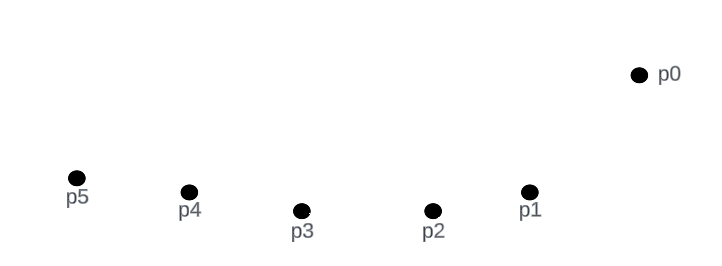
\includegraphics[width=0.7\linewidth]{tocke.png}
    \caption{Permutirane vhodne točke.}
    \label{tocke}
\end{figure}

Na vsakem koraku zanke, bo algoritem povezal najbolj desno točko, ki še ni bila povezana z ogljišči trikotnika v katerem je.

\begin{figure}[h!]
    \centering
    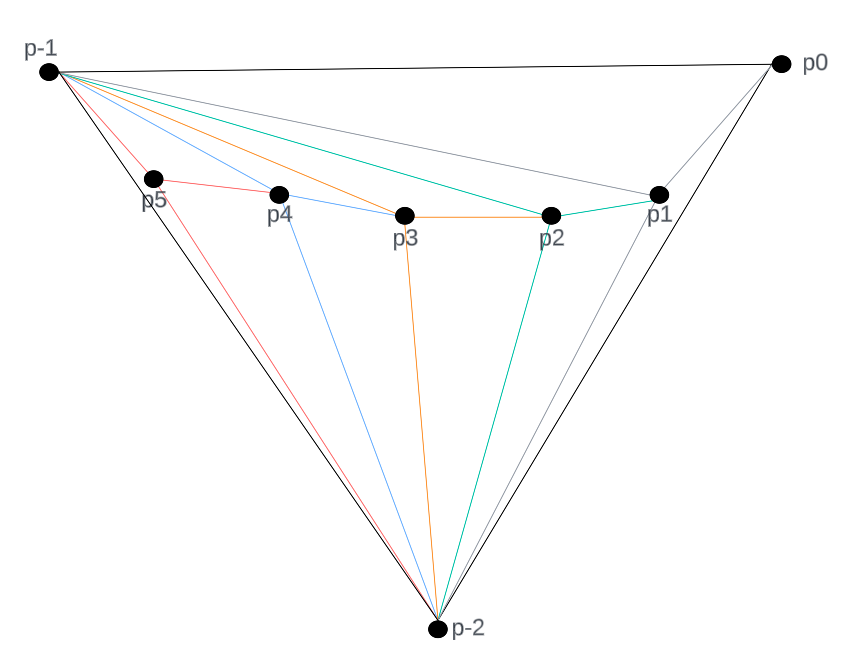
\includegraphics[width=0.7\linewidth]{triangulizacija.png}
    \caption{Delaunay triangualizacija.}
    \label{Delaunay}
\end{figure}

Istočasno pa gradi usmerjen acikličen graf $\mathcal{D}$, ki nosi informacijo o trenutnih in uničenih trikotnikih.
Ker točke dodaja vsakič znotraj najbolj levega trikotnika, bodo novi listi na grafu dodani vsakih pod istimi vozlišči, tako da bo končen graf neuravnovešen.

\begin{figure}[h!]
    \centering
    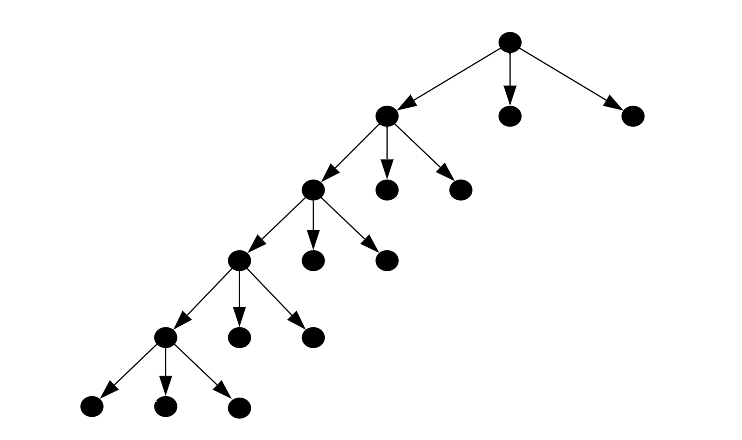
\includegraphics[width=0.7\linewidth]{graf.png}
    \caption{Usmerjen acikličen graf.}
    \label{graf}
\end{figure}

Na vsakem koraku mora algoritem najti kam postaviti novo točko. Ker je graf $\mathcal{D}$ vse bolj neuravnovešen, bo za iskanje porabil vse več časa.
Za prvo točko mora pregledati le tri vozlišča (liste pod korenom).
Za drugo jih mora pregledati šest.
Za $k$-to točko bo moral pregledati $3k$ vozlišč.
To mora narediti za vsako točko, torej bo za vsako od $n$ točk porabil $\mathcal{O} (n)$ časa, kar nam da časovno zahtevnost $\mathcal{O} (n^2)$.


\pagebreak
\section*{Naloga 3: Drevesne strukture}

\subsection*{Prednosti drevesnih struktur}

Četrtinska drevesa lahko uporabimo za kompresijo slik. Kompresija najbolje deluje za slike, ki imajo velike dele iste barve, saj namesto $k \times k$ kvadratov shrani samo enega.

Kd-drevesa so uravnotežena binarna drevesa, zato imajo logaritemsko globino in so najprimernejša za hitro iskanje najbližjih sosedov. Dobro delujejo tudi za sparse točke, saj se logaritemska globina ohrani, medtem ko je pri četrtinskih drevesih veliko praznega prostora.???

Intervalna drevesa so primerna za spreminjajča se podatke, na primer premikajoče točke. Namreč drevesna struktura se pri dodajanju in odstranjevanju točk ohrani, medtem ko se struktura četrtinskih dreves in kd-dreves spremeni toliko, da je lažje izdelati novo drevo.

\subsection*{Osmiška drevesa}

Podane imamo točke $P$ v $3$-dimenzionalnem prostoru. 
Prostor razdelimo na osem kock.
Nadaljne delitve prostora potekajo rekurzivno. 
Če je v kocki kvečemu ena točka, kocke ne delimo naprej.
Če je v kocki več kot ena točka, jo ponovno razdelimo na osem manjših kock in rekurzivno ponovimo na vseh novih otrocih.
Podrobneje je algoritem sledeč.

\vspace{2mm}
\noindent
\textcolor{gray}{(* Naj bodo točke predstavljene kot podatkovna struktura POINT(x, y, z). *)} \\
\textbf{struct POINT} (x, y, z)

\vspace{3mm}
\noindent
\textcolor{gray}{(* Naj bodo vozlišča predstavljena kot par (position, data), kjer prvi element predstavlja pozicijo v prostoru (kot točka), drugi pa vrednost, ki jo vozlišče nosi. *)} \\
\textbf{struct NODE} (position, data) 

\vspace{3mm}
\noindent
\textcolor{gray}{(* Definirajmo novo podatkovno strukturo Box, ki bo rekurzivno gradila Osmiško drevo. *)} \\
\textbf{struct BOX} (leftTopBack, rightBottomFront, maxCapacity): 

\textcolor{gray}{(* leftTopBack in rightBottomFront sta ustrezni}

\textcolor{gray}{nasprotni točki na diagonali kocke. *)}

\vspace{3mm}
\textcolor{gray}{(* Otroci (manjše kocke) so na začetku prazni. *)} 

leftTopBackBox = None 

leftTopFrontBox = None 

leftBottomBackBox = None 

leftBottomFrontBox = None 

rightTopBackBox = None 

rightTopFrontBox = None 

rightBottomBackBox = None 

rightBottomFrontBox = None

\vspace{3mm}
\textcolor{gray}{(*Točke shranjene v vozlišču.*)} 

points = [ ]

\vspace{3mm}
\textcolor{gray}{(* Funkcija za vstavljanje novih vozlišč. *)} 

\textbf{define insert} (node):

\vspace{3mm}
\hspace{1cm} \textcolor{gray}{(*Če je pozicija izven mej kocke, ne naredimo nič.*)} 

\hspace{1cm}  \textbf{if} node.position.x < leftTopBack.x \textbf{or} 

\hspace{1.6cm}  node.position.x > rightBottomFront.x \textbf{or} 

\hspace{1.6cm} node.position.y > leftTopBack.y \textbf{or}

\hspace{1.6cm} node.position.y < rightBottomFront.y \textbf{or}

\hspace{1.6cm} node.position.z > leftTopBack.z \textbf{or}

\hspace{1.6cm} node.position.z > leftTopBack.z :

\hspace{2cm} \textbf{do nothing}

\vspace{3mm}
\hspace{1cm} \textcolor{gray}{(*Če smo dosegli najmanjšo možno velikost kocke,} 

\hspace{1cm} \textcolor{gray}{shranimo vozlišče, če je v kocki še prostor.*)} 

\hspace{1cm}  \textbf{if} points.size < maxCapacity:

\hspace{2cm} \textbf{points.append(node)}

\vspace{3mm}
\hspace{1cm} \textcolor{gray}{(*Sicer pa preverimo v katero manjšo kocko spada.*)} 

\vspace{2mm}
\hspace{1cm} \textcolor{gray}{(*Točka je na levem delu.*)} 

\vspace{2mm}
\hspace{1cm}  \textbf{if} $\frac{\text{leftTopBack.x + rightBottomFront.x}}{2} \geq$ node.position.x:

\vspace{2mm}
\hspace{2cm} \textcolor{gray}{(*Točka je na sprednjem delu.*)} 

\vspace{2mm}
\hspace{2cm}  \textbf{if} $\frac{\text{leftTopBack.y + rightBottomFront.y}}{2} \geq$ node.position.y:

\vspace{2mm}
\hspace{3cm} \textcolor{gray}{(*Točka je na spodnjem delu.*)} 

\vspace{2mm}
\hspace{3cm}  \textbf{if} $\frac{\text{leftTopBack.z + rightBottomFront.z}}{2} \geq$ node.position.z:

\hspace{4cm} \textbf{leftBottomFrontBox.insert(node)}

\vspace{2mm}
\hspace{3cm} \textcolor{gray}{(*Točka je na zgornjem delu.*)} 

\vspace{2mm}
\hspace{3cm}  \textbf{else}: 

\hspace{4cm} \textbf{leftTopFrontBox.insert(node)}

\vspace{2mm}
\hspace{2cm} \textcolor{gray}{(*Točka je na zadnjem delu.*)} 

\vspace{2mm}
\hspace{2cm}  \textbf{else}: 


\vspace{2mm}
\hspace{3cm} \textcolor{gray}{(*Točka je na spodnjem delu.*)} 

\vspace{2mm}
\hspace{3cm}  \textbf{if} $\frac{\text{leftTopBack.z + rightBottomFront.z}}{2} \geq$ node.position.z:

\hspace{4cm} \textbf{leftBottomBackBox.insert(node)}

\vspace{2mm}
\hspace{3cm} \textcolor{gray}{(*Točka je na zgornjem delu.*)} 

\vspace{2mm}
\hspace{3cm}  \textbf{else}: 

\hspace{4cm} \textbf{leftTopBackBox.insert(node)}

\vspace{2mm}
\hspace{1cm} \textcolor{gray}{(*Točka je na desnem delu.*)} 

\vspace{2mm}
\hspace{1cm}  \textbf{else:}

\vspace{2mm}
\hspace{2cm} \textcolor{gray}{(*Točka je na sprednjem delu.*)} 

\vspace{2mm}
\hspace{2cm}  \textbf{if} $\frac{\text{leftTopBack.y + rightBottomFront.y}}{2} \geq$ node.position.y:

\vspace{2mm}
\hspace{3cm} \textcolor{gray}{(*Točka je na spodnjem delu.*)} 

\vspace{2mm}
\hspace{3cm}  \textbf{if} $\frac{\text{leftTopBack.z + rightBottomFront.z}}{2} \geq$ node.position.z:

\hspace{4cm} \textbf{rightBottomFrontBox.insert(node)}

\vspace{2mm}
\hspace{3cm} \textcolor{gray}{(*Točka je na zgornjem delu.*)} 

\vspace{2mm}
\hspace{3cm}  \textbf{else}: 

\hspace{4cm} \textbf{rightTopFrontBox.insert(node)}

\vspace{2mm}
\hspace{2cm} \textcolor{gray}{(*Točka je na zadnjem delu.*)} 

\vspace{2mm}
\hspace{2cm}  \textbf{else}: 


\vspace{2mm}
\hspace{3cm} \textcolor{gray}{(*Točka je na spodnjem delu.*)} 

\vspace{2mm}
\hspace{3cm}  \textbf{if} $\frac{\text{leftTopBack.z + rightBottomFront.z}}{2} \geq$ node.position.z:

\hspace{4cm} \textbf{rightBottomBackBox.insert(node)}

\vspace{2mm}
\hspace{3cm} \textcolor{gray}{(*Točka je na zgornjem delu.*)} 

\vspace{2mm}
\hspace{3cm}  \textbf{else}: 

\hspace{4cm} \textbf{rightTopBackBox.insert(node)}




\end{document}